% ============================================================
%  DDAA: A Large-Scale Real-World Benchmark for Deepfake Audio
%  Detection Under Acoustic Degradation and Adversarial Conditions
%  arXiv preprint version — de-anonymized
%  DO NOT submit this file to NeurIPS portal (use paper5_ddaa_benchmark.tex)
% ============================================================
\documentclass{article}

\usepackage[preprint]{neurips_2026}

\usepackage[utf8]{inputenc}
\usepackage[T1]{fontenc}
\usepackage{microtype}
\usepackage{booktabs}
\usepackage{amsmath,amssymb}
\usepackage{graphicx}
\usepackage{hyperref}
\usepackage{url}
\usepackage{xcolor}
\usepackage{multirow}
\usepackage{nicefrac}
\usepackage{makecell}
\usepackage{caption}
\captionsetup{font=small,skip=4pt,belowskip=0pt}
\usepackage{float}

\newcommand{\ddaa}{\textsc{DDAA}}
\newcommand{\figw}{0.78\linewidth}
\newcommand{\etal}{\textit{et al.}}
\newcommand{\eg}{\textit{e.g.,}}
\newcommand{\ie}{\textit{i.e.,}}
% Gray [TBD] for entries pending cluster jobs (remove before final submission)
\newcommand{\tbd}{\textcolor{gray}{[TBD]}}
% Placeholder box for figures not yet downloaded from cluster
\newcommand{\figplaceholder}[2]{%
  \fbox{\parbox{#1}{\centering\vspace{6pt}\small\texttt{#2}\vspace{6pt}}}}

% ============================================================
\title{\ddaa: A Large-Scale Real-World Benchmark for Deepfake Audio\\
  Detection Under Acoustic Degradation and Adversarial Conditions}

\author{%
  Matthew Sahagun \\
  Yale University \\
  \texttt{ms4726@yale.edu}
  \And
  Charlie Grube \\
  University of Connecticut \\
  \texttt{charlie.grube@uconn.edu}
}

\begin{document}
\maketitle

% ============================================================
\begin{abstract}
We show that strong deepfake audio detectors, evaluated under our protocol,
do not reliably generalize to synthesis systems held out from training.
Across six architectures (eight configurations) covering graph attention,
Kolmogorov--Arnold splines, a physics-informed head, and a neural ODE,
held-out evaluation on Bark, MMS-TTS, and SpeechT5 yields no AUC strictly
above 0.75 (maximum observed: 0.749); nine of fifteen
detector$\times$generator cells fall at or near chance.
\textbf{\ddaa} (\textbf{D}eepfake \textbf{D}etection \textbf{A}udio \textbf{A}rchive)
is a 449,847-sample benchmark designed to support evaluative claims about
detector behavior under \emph{realistic codec and channel degradation} and
\emph{generator shift}: paired Mozilla Common Voice utterances with neural TTS
and voice conversion, a stochastic degradation pipeline on every sample
(70\% lossy codec: MP3, Opus, AAC; 60\% channel effects: mobile band-limiting,
noise, reverberation), and voice-disjoint splits (16 in-domain synthesis
configurations across two paradigms).
We benchmark eight model configurations under five conditions:
in-distribution performance, held-out generators, cross-dataset transfer,
adversarial robustness, and degradation-stratified analysis.
A bidirectional domain gap separates \ddaa{} and ASVspoof~2019~LA: models
trained on \ddaa{} reach only 0.34--0.55 AUC zero-shot on ASVspoof, while
ASVspoof-pretrained baselines reach 0.452--0.584 AUC zero-shot on \ddaa{};
further ASVspoof fine-tuning of RawNet2 produces AUC~0.032 on \ddaa{}
(label inversion).
Our dataset and evaluation code are released under CC~BY~4.0; our trained
baseline checkpoints are released under the same terms where we hold
distribution rights, while upstream foundation weights (\textit{e.g.}, wav2vec~2.0)
remain under their original licenses.
\end{abstract}

% ============================================================
\section{Introduction}
\label{sec:intro}

Real-world deepfake audio does not arrive as a clean WAV file.  It is
synthesized, compressed to Opus at 16~kbps by a messaging app, transmitted
over a noisy VoIP channel, and played back through a phone speaker.  The
canonical anti-spoofing benchmark, ASVspoof~2019~LA
\citep{asvspoof2019}, evaluates under none of these conditions.  Its
training data is studio-quality; its synthesis systems are a fixed,
known set; and its test split shares speakers with training data in some
configurations.  Progress on ASVspoof EER therefore cannot be assumed
to transfer to real-world deployment---and experimentally, it does not.
Current detectors learn
\emph{generator-specific artifacts}: the spectral fingerprint of a
particular vocoder, the prosodic discontinuities of a specific
autoregressive model, the phase coherence signature of a codec-based
system.  When a detector encounters a generator it has not seen, it has
no artifacts to latch onto and performs near chance.
Table~\ref{tab:t2} documents this for five detectors across three
held-out synthesis systems: \emph{no point estimate strictly exceeds
AUC~0.750} (maximum $0.749$, with approximate intervals in-table).

We introduce \ddaa{} to expose and measure this gap at scale.
The design differs from prior benchmarks in three ways.
First, degradation is applied at training time: real and synthetic audio both
pass through the same stochastic codec and channel pipeline, so models cannot
use compression artifacts as a proxy label.
Second, 16 training systems span two synthesis paradigms---neural TTS
(Edge-TTS, 10 voices across US/AU/GB/IN accents) and voice conversion (RVC,
6 public-figure voice clones)---while Bark, MMS-TTS, and SpeechT5 are held
out for generalization evaluation (Section~\ref{sec:generalization}).
Third, all splits are voice-disjoint: no speaker ID appears in more than one
partition, which forces generalization over voice characteristics rather than
speaker identity.

\paragraph{Contributions.}
\begin{itemize}
  \item \ddaa: 449,847 labeled utterances across 16 TTS/VC configurations
  (10 Edge-TTS voices, 6 RVC models) spanning neural TTS and voice conversion,
  with a realistic degradation pipeline applied symmetrically to all audio.
  The largest publicly released benchmark of its kind.
  \item An evaluation suite covering six architectures under five conditions,
  with bootstrap CIs, DET curves, min-tDCF, and per-paradigm EER breakdown.
  \item A standardized measurement of the cross-architecture generalization gap:
  under our held-out generator protocol, no point-estimate AUC strictly exceeds
  $0.75$ (maximum $0.749$); approximate confidence intervals are reported in
  Table~\ref{tab:t2}.
\end{itemize}

% ============================================================
\section{Related Work}
\label{sec:related}

\paragraph{Anti-spoofing benchmarks.}
ASVspoof~2019~LA \citep{asvspoof2019} remains the standard, with 19 TTS/VC
systems synthesized from VCTK.  ASVspoof~2021~LA \citep{asvspoof2021} added
codec degradation to the \emph{evaluation} set only, leaving training clean.
ADD \citep{yi2022add} and ADD~2.0 \citep{yi2023add2} introduced partially
faked utterances.  FakeAVCeleb \citep{khalid2021fakeavceleb} targets
audio-visual deepfakes.  In-the-Wild \citep{muller2022does} collected real
deepfakes from public media ($\sim$37k utterances) but provides no
standardized training split.  WaveFake \citep{frank2021wavefake} covers
six neural vocoders on LJSpeech but applies no degradation and fixes the
real-audio source to a single speaker.  Table~\ref{tab:benchmark_compare}
summarizes how \ddaa{} differs from all prior benchmarks on the axes most
relevant to real-world deployment.

\begin{table}[h]
  \caption{Comparison of deepfake audio benchmarks. \textbf{Train Degraded}:
  codec/channel effects applied to the \emph{training} split.
  \textbf{V-Disjoint}: no speaker appears in more than one split.
  \textbf{Open}: publicly downloadable under a permissive license.
  $\dagger$~ASVspoof~2021 degrades the \emph{eval} set only.
  $\ddagger$~In-the-Wild has no standardized training split.}
  \label{tab:benchmark_compare}
  \centering
  \small
  \setlength{\tabcolsep}{4.5pt}
  \begin{tabular}{lrrllll}
    \toprule
    Dataset & Samples & Systems & Train Degraded & V-Disjoint & Open & License \\
    \midrule
    ASVspoof 2019 LA \citep{asvspoof2019}  & 121,461  & 19 & No              & No  & Restricted & Custom \\
    ASVspoof 2021 LA \citep{asvspoof2021}  & 181,566  & 13 & No$^\dagger$    & No  & Restricted & Custom \\
    ADD 2.0 \citep{yi2023add2}             &   4,000  & 10 & No              & No  & No         & ---    \\
    WaveFake \citep{frank2021wavefake}     & 117,985  &  6 & No              & N/A & Yes        & MIT    \\
    In-the-Wild \citep{muller2022does}     &  37,176  & ?  & No$^\ddagger$   & No  & Yes        & CC BY 4.0 \\
    FakeAVCeleb \citep{khalid2021fakeavceleb} & 19,500 & 4 & No             & No  & Yes        & CC BY 4.0 \\
    \midrule
    \textbf{\ddaa{} (ours)}                & \textbf{449,847} & \textbf{16} & \textbf{Yes} & \textbf{Yes} & \textbf{Yes} & \textbf{CC BY 4.0} \\
    \bottomrule
  \end{tabular}
\end{table}

No prior benchmark degrades the training split, enforces voice-disjoint
partitioning, \emph{and} covers voice conversion alongside neural TTS---the
two paradigms most prevalent in real-world deepfake audio---while holding out
unseen synthesis systems for generalization evaluation.  \ddaa{} does all three.

\paragraph{Detection architectures.}
AASIST \citep{jung2022aasist} and RawNet2 \citep{tak2021end} lead on ASVspoof;
raw-waveform and conformer variants \citep{ge2021raw,martin2022vicomtech} improve robustness to channel mismatch.
We compare them on \ddaa{} alongside KAN splines \citep{liu2024kan,liu2024kan2}, PINN-style temporal constraints
\citep{raissi2019physics}, Transformer, and a frame-controlled Neural ODE \citep{chen2018neural} (RK4, standard backprop through the solver)---to our knowledge the first such head-to-head on a single \emph{train-time} degraded benchmark.

\paragraph{Codec robustness.}
Prior work on codec effects in spoofing detection
\citep{das2020attacker,shi2020robust} is small-scale.
\ddaa's 449,847 samples, each with a recorded codec configuration, make
systematic analysis of compression-specific detection difficulty possible
for the first time.

% ============================================================
\section{Dataset Construction}
\label{sec:dataset}

\subsection{Real Audio Source}

Real speech is drawn from \textbf{Mozilla Common Voice 24.0}
(\texttt{cv-corpus-24.0-2025-12-05}, English), which provides permissive
CC0 licensing and broad speaker demographic diversity.  We selected
utterances from \textbf{2,847 unique speakers}, partitioned into
train/val/test sets with \textbf{zero speaker overlap}---speaker IDs are
strictly disjoint across all splits.  Average utterance duration is 4.7~s
($\sigma = 1.8$~s) before truncation; all audio is zero-padded or truncated
to 5~s (80,000 samples at 16~kHz) for model input.

\subsection{Synthesis Systems}
\label{sec:synthesis}

We synthesize a fake counterpart for each real utterance using 16 TTS/VC
systems across two paradigms (Table~\ref{tab:systems}).  Three additional
systems---Bark, MMS-TTS, SpeechT5---are reserved as held-out generators
for generalization evaluation (Section~\ref{sec:generalization}).

\paragraph{Neural TTS (non-autoregressive).}
\textbf{Edge-TTS} \citep{microsoftedge} with ten voices spanning four
English accent regions:
en-US (\texttt{GuyNeural}, \texttt{JennyNeural}, \texttt{AriaNeural},
\texttt{ChristopherNeural}),
en-AU (\texttt{NatashaNeural}, \texttt{WilliamNeural}),
en-GB (\texttt{RyanNeural}, \texttt{SoniaNeural}),
en-IN (\texttt{NeerjaNeural}, \texttt{PrabhatNeural}).
Edge-TTS uses HiFi-GAN-based neural vocoders; its artifacts concentrate in
high-frequency spectral fine structure.

\paragraph{Voice Conversion (RVC).}
Six Retrieval-based Voice Conversion \citep{rvc2023} models with public
figure voice clones: Biden, Trump, Taylor Swift, Kanye West, Ed Sheeran,
Obama.
RVC preserves the real speaker's macro-level prosody and rhythm, making it
particularly deceptive: synthesis artifacts are largely confined to timbre
and spectral envelope, while timing and intonation are real.  Micro-level
discontinuities---phase irregularities and spectral envelope mismatches at
phoneme boundaries---are introduced by the voice conversion pipeline and
constitute the primary detection signal at speech onset.

\begin{table}[h]
  \caption{Training synthesis systems in \ddaa{} by paradigm.
  Bark, MMS-TTS, and SpeechT5 are held out for generalization evaluation.}
  \label{tab:systems}
  \centering
  \small
  \begin{tabular}{llrc}
    \toprule
    Paradigm & Systems & Count & Total \\
    \midrule
    Neural TTS & Edge-TTS $\times$10 (US/AU/GB/IN accents) & 10 & \\
    Voice Conversion (RVC) & Biden, Trump, T.\ Swift, K.\ West, Ed Sheeran, Obama & 6 & \\
    \midrule
    \textbf{Total (training)} & & & \textbf{16} \\
    \bottomrule
  \end{tabular}
\end{table}

\subsection{Acoustic Degradation Pipeline}

Each utterance draws independently from two stochastic tiers; paired
real/fake samples share an RNG seed so counterfeits cannot be separated by
channel draw alone.  After degradation, all audio is resampled to 16~kHz and
zero-padded/truncated to 5~s (80,000 samples); applying the same pipeline to
real audio prevents codec/channel artifacts from leaking labels.

\begin{table}[h]
  \caption{Per-utterance degradation mixtures (probabilities sum to 100\%
  within each tier).}
  \label{tab:degradation}
  \centering
  \footnotesize
  \begin{tabular}{@{}p{0.14\linewidth}p{0.80\linewidth}@{}}
    \toprule
    Codec &
      30\% clean;\,
      20\% MP3 (64\,kbps);\,
      20\% Opus (48\,kbps);\,
      15\% AAC (96\,kbps);\,
      15\% AAC (128\,kbps). \\
    Channel &
      40\% clean;\,
      40\% mobile (7\,kHz LP, 30\,dB SNR);\,
      20\% noisy tel.\ (5\,kHz LP, 15\,dB SNR, McDermott RIR
      \citep{traer2016statistics}). \\
    \bottomrule
  \end{tabular}
\end{table}

\subsection{Dataset Statistics}

\begin{table}[h]
  \caption{\ddaa{} split statistics. Class imbalance (62\% real / 38\%
  synthetic) reflects the fact that 16 synthetic systems generate one sample
  per real utterance, but not all speakers have equal coverage across all
  systems. Voice-disjoint: no speaker ID appears in more than one split.}
  \label{tab:stats}
  \centering
  \begin{tabular}{lrrrr}
    \toprule
    Split & Total & Speakers & Real & Synthetic \\
    \midrule
    Train      & 317,935 & 2,277 & 197,871 & 120,064 \\
    Validation &  70,109 &   284 &  43,661 &  26,448 \\
    Test       &  61,803 &   286 &  38,437 &  23,366 \\
    \midrule
    \textbf{Total} & \textbf{449,847} & \textbf{2,847} &
      \textbf{279,969} & \textbf{169,878} \\
    \bottomrule
  \end{tabular}
\end{table}

% ============================================================
\section{Dataset Analysis}
\label{sec:analysis_data}

\paragraph{Per-TTS-system difficulty.}
Figure~\ref{fig:per_tts_eer} shows per-synthesis-paradigm EER for all
fine-tuned detectors.  Voice conversion systems (RVC) are
consistently the hardest to detect, followed by neural TTS (Edge-TTS).
This ranking is \emph{consistent across all fine-tuned detectors}, confirming
that difficulty is a property of the synthesis paradigm, not the detector
architecture.

\begin{figure}[ht]
  \centering
  \includegraphics[width=\figw]{figures/fig5_per_tts_eer.png}
  \caption{EER by synthesis paradigm (\ddaa{} test). RVC hardest, Edge-TTS easiest;
  held-out Bark near-random (EER~47--58\%).}
  \label{fig:per_tts_eer}
\end{figure}

\paragraph{Spectrograms.}
Representative mel-spectrograms after codec compression are shown in
Appendix~\ref{fig:spectrograms}.  Neural TTS (Edge-TTS) artifacts appear as
spectral smoothing in the 4--8~kHz band; RVC samples are visually nearly
indistinguishable from real audio, consistent with higher EER for voice
conversion across detectors.

% ============================================================
\section{Experimental Setup}
\label{sec:setup}

\paragraph{Models.}
We evaluate eight model configurations (six architectures, two evaluated
both zero-shot and fine-tuned).
\textbf{AASIST} \citep{jung2022aasist}: heterogeneous
graph attention network over raw waveform and spectral branches; evaluated
zero-shot (ASVspoof pre-trained weights, no \ddaa{} training) and
fine-tuned on \ddaa{} training split.  \textbf{RawNet2} \citep{tak2021end}:
sinc-filter front-end + residual GRU; same zero-shot / fine-tuned evaluation.
The four novel architectures all share a \textbf{wav2vec~2.0 base encoder}
\citep{baevski2020wav2vec} fine-tuned end-to-end with differential learning rates:
\textbf{Transformer} (125M parameters total), \textbf{KAN} (35.5M, grid~5,
spline order~5) \citep{liu2024kan}, \textbf{PINN} (30.8M, temporal
smoothness physics loss with $\lambda{=}0.05$) \citep{raissi2019physics},
and \textbf{Neural ODE}
(30.2M; frame-controlled continuous-time latent dynamics via RK4 integration
\citep{chen2018neural}).
All novel models trained with AdamW, cosine annealing, gradient clipping,
and early stopping on validation AUC.

\paragraph{Metrics.}
\textbf{AUC-ROC} is the primary ranking metric.  We also report
\textbf{EER}, \textbf{Accuracy}, \textbf{F1-Macro}, and
\textbf{min-tDCF} (Table~\ref{fig:mintdcf}) for comparability with ASVspoof
submissions.  Bootstrap confidence intervals (1,000 resamples, 95\% CI) are
in Table~\ref{fig:bootstrap}.

\paragraph{Evaluation conditions.}
(1)~\textbf{In-distribution}: full \ddaa{} test set (61,803 samples).
(2)~\textbf{Cross-architecture generalization}: hold-one-system-out; models
evaluated on the 3 generators never seen during training (Bark, MMS-TTS,
SpeechT5).
(3)~\textbf{Cross-dataset transfer}: \ddaa-trained models evaluated on
ASVspoof~2019~LA eval set; ASVspoof-pretrained models evaluated on \ddaa{}.
(4)~\textbf{Adversarial robustness}: FGSM, PGD ($\varepsilon$=0.01), and
CleverHans \citep{papernot2018cleverhans} psychoacoustic attack on 1,000 test samples.
(5)~\textbf{Degradation robustness}: stratified by codec/channel condition.

% ============================================================
\section{Results}
\label{sec:results}

\subsection{In-Distribution Performance}

\begin{table}[ht]
  \caption{In-distribution results on the \ddaa{} held-out test set
  (61,803 samples, 62\% real / 38\% synthetic).
  \textbf{FT} = fine-tuned on \ddaa{}. \textbf{ZS} = zero-shot
  (ASVspoof pre-trained weights only, no \ddaa{} training).
  Models sorted by AUC.}
  \label{tab:t1}
  \centering
  \setlength{\tabcolsep}{5.5pt}
  \begin{tabular}{llcccc}
    \toprule
    Model & Setup & AUC $\uparrow$ & EER $\downarrow$ &
      Acc $\uparrow$ & F1-Mac $\uparrow$ \\
    \midrule
    PINN        & FT (\ddaa)             & \textbf{97.6\%} & 7.9\%  & 96.9\% & 96.6\% \\
    KAN         & FT (\ddaa)             & 97.2\%          & 7.3\%  & 93.1\% & 92.5\% \\
    AASIST      & FT (\ddaa)             & 95.3\%          & 11.8\% & 87.6\% & 73.9\% \\
    Neural ODE  & FT (\ddaa)             & 92.2\%          & 14.3\% & 87.6\% & 85.4\% \\
    Transformer & FT (\ddaa)             & 89.0\%          & 22.4\% & 90.4\% & 89.2\% \\
    RawNet2     & FT (\ddaa)             & 87.8\%          & 17.9\% & 81.8\% & 81.0\% \\
    \midrule
    AASIST      & ZS (ASVspoof weights)  & 58.4\%          & 42.5\% & 61.2\% & ---    \\
    RawNet2     & ZS (ASVspoof weights)  & 45.2\%          & 52.7\% & 50.8\% & ---    \\
    \bottomrule
  \end{tabular}
\end{table}

The task is learnable: PINN reaches 97.6\% AUC and 96.9\% accuracy when
trained on in-distribution data.  The zero-shot baselines tell a different
story.  RawNet2, applied directly with ASVspoof-pretrained weights, reaches
only 45.2\% AUC---\emph{worse than random}---and AASIST fares little better at
58.4\%.  ASVspoof pretraining transfers nothing useful to \ddaa{} detection,
the first direction of the bidirectional gap described in Section~\ref{sec:generalization}.

\begin{figure}[ht]
  \centering
  \includegraphics[width=\figw]{figures/fig2_score_distributions.png}
  \caption{Score distributions (\ddaa{} test). PINN/KAN FT bimodal; RawNet2/AASIST ZS overlap (AUC~0.45--0.58).}
  \label{fig:score_dist}
\end{figure}

\begin{figure}[ht]
  \centering
  \includegraphics[width=\figw]{figures/fig3_det_curves.png}
  \caption{DET curves (eight detectors); ZS baselines near diagonal (chance on \ddaa{}).}
  \label{fig:det}
\end{figure}

\begin{table}[ht]
  \caption{Bootstrap 95\% CIs (1{,}000 resamples) for AUC and EER on the \ddaa{}
  test set. PINN/KAN intervals do not overlap lower-ranked models.}
  \label{fig:bootstrap}
  \centering
  \footnotesize
  \setlength{\tabcolsep}{4pt}
  \begin{tabular}{lcccc}
    \toprule
    Model & AUC mean & AUC 95\% CI & EER mean (\%) & EER 95\% CI (\%) \\
    \midrule
    PINN        & 0.9763 & [0.9751, 0.9773] &  7.91 & [7.67, 8.17] \\
    KAN         & 0.9720 & [0.9706, 0.9733] &  7.35 & [7.12, 7.54] \\
    AASIST      & 0.9529 & [0.9513, 0.9543] & 11.79 & [11.55, 12.04] \\
    NeuralODE   & 0.9218 & [0.9195, 0.9241] & 14.32 & [14.01, 14.65] \\
    Transformer & 0.8897 & [0.8870, 0.8924] & 22.38 & [21.97, 22.81] \\
    RawNet2~FT  & 0.8768 & [0.8739, 0.8795] & 17.85 & [17.55, 18.12] \\
    RawNet2~ZS  & 0.4219 & [0.4171, 0.4265] & 55.80 & [55.39, 56.20] \\
    AASIST~ZS   & 0.5843 & [0.5796, 0.5890] & 42.52 & [42.13, 42.92] \\
    \bottomrule
  \end{tabular}
\end{table}

\begin{table}[ht]
  \caption{Minimum tandem Decision Cost Function (min-tDCF) for all detectors,
  computed using ASVspoof 2019~LA cost parameters ($C_\mathrm{miss}=1$,
  $C_\mathrm{fa}=10$, $P_\mathrm{target}=0.05$). Lower is better.
  Models at the min-tDCF floor (0.0500) are constrained by the cost
  function ceiling, not by detector quality.}
  \label{fig:mintdcf}
  \centering
  \small
  \setlength{\tabcolsep}{6pt}
  \begin{tabular}{lcccc}
    \toprule
    Model & AUC & EER (\%) & EER Threshold & min-tDCF \\
    \midrule
    PINN        & 0.9763 &  7.91 & 0.0006 & \textbf{0.0198} \\
    KAN         & 0.9720 &  7.35 & 0.0140 & 0.0294 \\
    AASIST      & 0.9529 & 11.78 & 0.1782 & 0.0483 \\
    NeuralODE   & 0.9218 & 14.32 & 0.8267 & 0.0500 \\
    Transformer & 0.8897 & 22.38 & 0.0149 & 0.0312 \\
    RawNet2~FT  & 0.8768 & 17.84 & 0.2710 & 0.0500 \\
    RawNet2~ZS  & 0.4219 & 55.79 & 0.0017 & 0.0500 \\
    AASIST~ZS   & 0.5844 & 42.51 & 0.1046 & 0.0500 \\
    \bottomrule
  \end{tabular}
\end{table}

\subsection{Cross-Architecture Generalization}
\label{sec:generalization}

\begin{table}[ht]
  \caption{Cross-architecture generalization (AUC-ROC) on held-out generators
  (Bark $n{=}500$; MMS-TTS, SpeechT5 $n{=}2{,}000$ each). Brackets: approximate
  95\% AUC CIs (Hanley--McNeil \citep{hanley1982auc}). \textbf{No point estimate
  strictly exceeds 0.750} (AASIST/SpeechT5 $0.749$, upper CI $0.764$).}
  \label{tab:t2}
  \centering
  \small
  \setlength{\tabcolsep}{5pt}
  \begin{tabular}{lccc}
    \toprule
    Detector & Bark & MMS-TTS & SpeechT5 \\
             & ($n$=500) & ($n$=2{,}000) & ($n$=2{,}000) \\
    \midrule
    Transformer  & \makecell{0.485\\[-1pt]{\scriptsize [0.450, 0.521]}} & \makecell{0.325\\[-1pt]{\scriptsize [0.309, 0.342]}} & \makecell{0.271\\[-1pt]{\scriptsize [0.255, 0.286]}} \\
    KAN          & \makecell{0.568\\[-1pt]{\scriptsize [0.533, 0.604]}} & \makecell{0.378\\[-1pt]{\scriptsize [0.361, 0.395]}} & \makecell{0.430\\[-1pt]{\scriptsize [0.412, 0.447]}} \\
    PINN         & \makecell{0.441\\[-1pt]{\scriptsize [0.406, 0.477]}} & \makecell{0.394\\[-1pt]{\scriptsize [0.377, 0.412]}} & \makecell{0.567\\[-1pt]{\scriptsize [0.549, 0.585]}} \\
    AASIST (FT)  & \makecell{0.533\\[-1pt]{\scriptsize [0.497, 0.569]}} & \makecell{0.581\\[-1pt]{\scriptsize [0.564, 0.599]}} & \makecell{\textbf{0.749}\\[-1pt]{\scriptsize [0.734, 0.764]}} \\
    RawNet2 (FT) & \makecell{0.473\\[-1pt]{\scriptsize [0.437, 0.508]}} & \makecell{0.305\\[-1pt]{\scriptsize [0.289, 0.322]}} & \makecell{0.671\\[-1pt]{\scriptsize [0.654, 0.687]}} \\
    \midrule
    \multicolumn{4}{l}{\textit{Chance: 0.500}} \\
    \bottomrule
  \end{tabular}
\end{table}

\textbf{Across five detectors and three held-out synthesis systems, no point
estimate exceeds $0.749$, and none strictly exceeds $0.750$.}
Nine of fifteen cells fall below or near chance,
and the failure spans every tested architecture---it is a property of current
detection methodology, not of any single model.

Four of five detectors share wav2vec~2.0; under shift the failure is at least partly
an SSL representation issue, while AASIST's SpeechT5 peak (0.749 vs.\ 0.27--0.57)
hints that raw-waveform graphs retain vocoder cues that SSL discards---we leave
systematic study of that split to future work.

\subsection{Cross-Dataset Transfer (Bidirectional Domain Gap)}

\begin{table}[ht]
  \caption{Cross-dataset transfer (ASVspoof~2019~LA). Blocks: \ddaa{}$\rightarrow$ASVspoof ZS;
  \ddaa{} models FT 10 epochs on ASVspoof LA then ASVspoof eval; ASVspoof-pretrained$\rightarrow$\ddaa{} ZS.
  $\dagger$~Label inversion (wrong class, not chance).}
  \label{tab:t3}
  \centering
  \setlength{\tabcolsep}{7pt}
  \begin{tabular}{llcc}
    \toprule
    Model & Condition & AUC & EER \\
    \midrule
    \multicolumn{4}{l}{\textit{\ddaa-trained $\rightarrow$ ASVspoof 2019 LA (zero-shot)}} \\
    Transformer & ZS on ASVspoof & 55.4\% & 44.0\% \\
    KAN         & ZS on ASVspoof & 51.1\% & 49.3\% \\
    Neural ODE  & ZS on ASVspoof & 45.1\% & 53.9\% \\
    PINN        & ZS on ASVspoof & 34.1\% & 63.7\% \\
    \midrule
    \multicolumn{4}{l}{\textit{\ddaa-trained $\rightarrow$ ASVspoof 2019 LA (fine-tuned)}} \\
    PINN        & FT on ASVspoof & \textbf{95.8\%} & 11.2\% \\
    KAN         & FT on ASVspoof & 83.6\% & 23.5\% \\
    Transformer & FT on ASVspoof & 72.9\% & 29.3\% \\
    \midrule
    \multicolumn{4}{l}{\textit{ASVspoof 2019 LA $\rightarrow$ \ddaa{} (reverse direction, zero-shot)}} \\
    AASIST  & ZS on \ddaa{} (ASVspoof pretrained)     & 58.4\% & 42.5\% \\
    RawNet2 & ZS on \ddaa{} (ASVspoof pretrained)     & 45.2\% & 52.7\% \\
    RawNet2 & FT on ASVspoof (5 epochs) $\rightarrow$ \ddaa{} & \textbf{3.2\%}$^\dagger$  & 91.1\% \\
    \midrule
    \multicolumn{4}{l}{\textit{ASVspoof-native baselines (trained and tested on ASVspoof)}} \\
    AASIST  & Native & $\approx$99.0\% & $\approx$0.83\% \\
    RawNet2 & Native & ---             & $\approx$4.0\%  \\
    \bottomrule
  \end{tabular}
\end{table}

Zero-shot transfer fails both ways (AUC~0.34--0.58).  ASVspoof-then-\ddaa{}
RawNet2 (5 epochs) inverts labels (AUC~\textbf{0.032}) while the same protocol
recovers PINN to 95.8\% \emph{on} ASVspoof---distribution shift, not capacity
(Figure~\ref{fig:finetuning}); \ddaa{} artifacts after codecs differ from clean-studio cues ASVspoof rewards.

\begin{figure}[ht]
  \centering
  \includegraphics[width=\figw]{figures/fig10_finetuning_curves.png}
  \caption{ASVspoof LA fine-tuning curves (DDAA init). PINN peaks 95.8\% AUC (epoch~9);
  dashed line: Phase~2 encoder unfreeze.}
  \label{fig:finetuning}
\end{figure}

\subsection{Adversarial Robustness}

\begin{table}[ht]
  \caption{Adversarial accuracy ($n{=}1{,}000$, $\varepsilon{=}0.01$; PGD-40; CleverHans masking \citep{papernot2018cleverhans}). PINN worst PGD; KAN best CleverHans.}
  \label{tab:t4}
  \centering
  \setlength{\tabcolsep}{5pt}
  \begin{tabular}{lcccc}
    \toprule
    Model & Clean Acc & FGSM Adv & PGD Adv & CleverHans Adv \\
    \midrule
    Transformer & 88.3\% & 67.0\% & 3.9\%  & 39.5\% \\
    KAN         & 90.9\% & 69.0\% & 23.1\% & \textbf{56.1\%} \\
    PINN        & 93.7\% & 71.6\% & \textbf{0.3\%}  & 18.8\% \\
    Neural ODE  & 91.3\% & 64.7\% & 26.5\% & 27.6\% \\
    \bottomrule
  \end{tabular}
\end{table}

FGSM causes only modest drops---all models hold 64--71\% accuracy---so
single-step perturbations at $\varepsilon=0.01$ are not sufficient to break
these detectors.  PGD is a different story for the PINN, which collapses to
0.3\% adversarial accuracy under 40-step attack.  The failure is
counterintuitive: the temporal smoothness constraint that shields the PINN
from natural degradation also structures the gradient landscape in a way that
iterative optimization can exploit cleanly.

CleverHans is the most practically relevant attack because it operates without
white-box access, and here KAN leads at 56.1\% adversarial accuracy.  The
B-spline activations appear to spread gradient information more diffusely
across input dimensions, which makes it harder to construct a single
perturbation direction that reliably fools the classifier.

\begin{figure}[ht]
  \centering
  \includegraphics[width=\figw]{figures/fig8_robustness_eps.png}
  \caption{Adv.\ accuracy vs.\ $\varepsilon$ (FGSM/PGD). PINN collapses under strong PGD;
  KAN best on CleverHans sweep.}
  \label{fig:robustness_eps}
\end{figure}

% ============================================================
\section{Discussion}
\label{sec:discussion}

\paragraph{Why does the domain gap exist?}
ASVspoof 2019~LA is studio-quality audio.  TTS artifacts in that setting
concentrate in high-frequency spectral fine structure above 4~kHz---the kind
of detail that neural vocoders leave behind in clean conditions.  \ddaa's
codec compression and telephony simulation wipe out that band.  A model
trained on ASVspoof arrives at \ddaa{} looking for fingerprints that no longer
exist.  Going the other direction is no easier: \ddaa-trained models learn to
detect artifacts in degraded signals, and those artifacts look nothing like the
clean spectrograms ASVspoof rewards.

Appendix Figs.~\ref{fig:attribution}--\ref{fig:ode} align with this story:
integrated gradients peak at speech onset/low formants; KAN spline energy sits in
mel bins 20--45 ($\sim$800--3000~Hz), the band codecs leave intact; ODE latent
trajectories separate fake from real more strongly at $t{=}1$ than at $t{=}0$
(see appendix for numeric Fisher/displacement summaries).

\paragraph{Synthesis paradigm as a stratification axis.}
Synthesis paradigm is a better predictor of detection difficulty than model
architecture.  Voice conversion (RVC) is consistently harder than neural TTS
(Edge-TTS) across all fine-tuned detectors, though the gap varies by model.
Bark, held out from training, lands near random EER (47--58\%) for all
architectures---a reminder that aggregate EER can look respectable while
hiding near-complete failure on specific synthesis types.  Breaking results
out by paradigm should be standard practice.

\paragraph{Limitations.}
\ddaa{} covers English only (Mozilla Common Voice English subset), which
limits what can be said about multilingual synthesis systems.  The 62\%/38\%
class imbalance makes accuracy a poor summary metric---AUC is used throughout
for this reason.  Training covers only two synthesis paradigms; diffusion-based
TTS, autoregressive language models like Bark, and low-resource vocoders are
held out as generalization targets but absent from training, so the benchmark
does not yet reflect the full range of synthesis methods in the wild.  Four of
the six architectures share a wav2vec~2.0 encoder, meaning comparisons among
them are largely comparisons of classification heads---adding raw-waveform and
spectrogram-CNN baselines would put the cross-architecture conclusions on
stronger footing.  The RVC voice clones are built from public-figure internet
audio, which may not be representative of real-world attacker pipelines.
Adversarial robustness uses 1{,}000-sample subsets; broader attack suites and a
clean-audio ablation of the degradation pipeline are deferred to future work.

% ============================================================
\section{Conclusion}
\label{sec:conclusion}

We introduced \ddaa, a 449,847-utterance benchmark that trains and evaluates
deepfake audio detectors under realistic codec compression and channel
degradation.  Three results stand out.  First, under our held-out generator
protocol (Table~\ref{tab:t2}), no AUC point estimate strictly exceeds $0.750$
(maximum $0.749$; approximate CIs in-table), across raw-waveform, SSL-based,
and physics-constrained representations alike---consistent with a shared
failure mode under generator shift rather than any single architectural fix.
Second, the domain gap between \ddaa{} and
ASVspoof is bidirectional: zero-shot transfer fails in both directions
(AUC 0.34--0.58), and further ASVspoof fine-tuning actively degrades \ddaa{}
performance via label inversion, confirming the two benchmarks measure
qualitatively different acoustic phenomena.  Third, synthesis paradigm
predicts detection difficulty more reliably than model architecture---voice
conversion (RVC) is consistently harder than neural TTS across all detectors,
and this ranking should be treated as a first-class stratification axis in
future benchmark design.  Our dataset and evaluation code are released under
CC~BY~4.0; baseline checkpoints we distribute use the same license where we
hold rights, while upstream foundation weights retain their original licenses.

% ============================================================
\begin{thebibliography}{99}
\small

\bibitem[Todisco et~al.(2019)]{asvspoof2019}
Todisco, M., et~al.
\newblock ASVspoof 2019: Future Horizons in Spoofed and Fake Audio Detection.
\newblock \textit{Interspeech}, 2019.

\bibitem[Delgado et~al.(2021)]{asvspoof2021}
Delgado, H., et~al.
\newblock ASVspoof 2021: Automatic Speaker Verification Spoofing and
  Countermeasures Challenge Evaluation Plan.
\newblock \textit{arXiv}:2109.00535, 2021.

\bibitem[Jung et~al.(2022)]{jung2022aasist}
Jung, J.-w., et~al.
\newblock AASIST: Audio Anti-Spoofing using Integrated Spectro-Temporal Graph
  Attention Networks.
\newblock \textit{ICASSP}, 2022.

\bibitem[Tak et~al.(2021)]{tak2021end}
Tak, H., et~al.
\newblock End-to-End Anti-Spoofing with RawNet2.
\newblock \textit{ICASSP}, 2021.

\bibitem[Chen et~al.(2018)]{chen2018neural}
Chen, R.~T.~Q., Rubanova, Y., Bettencourt, J., Duvenaud, D.
\newblock Neural Ordinary Differential Equations.
\newblock \textit{Advances in Neural Information Processing Systems (NeurIPS)}, 2018.

\bibitem[Liu et~al.(2024a)]{liu2024kan}
Liu, Z., et~al.
\newblock KAN: Kolmogorov-Arnold Networks.
\newblock \textit{arXiv}:2404.19756, 2024.

\bibitem[Liu et~al.(2024b)]{liu2024kan2}
Liu, Z., et~al.
\newblock KAN 2.0: Kolmogorov-Arnold Networks Meet Science.
\newblock \textit{arXiv}:2408.10205, 2024.

\bibitem[Raissi et~al.(2019)]{raissi2019physics}
Raissi, M., Perdikaris, P., Karniadakis, G.~E.
\newblock Physics-Informed Neural Networks.
\newblock \textit{Journal of Computational Physics}, 378:686--707, 2019.

\bibitem[Baevski et~al.(2020)]{baevski2020wav2vec}
Baevski, A., et~al.
\newblock wav2vec 2.0: A Framework for Self-Supervised Learning of Speech
  Representations.
\newblock \textit{NeurIPS}, 2020.

\bibitem[Wang \& Yamagishi(2022)]{wang2023review}
Wang, X., Yamagishi, J.
\newblock A Practical Guide to Logical Access Voice Presentation Attack
  Detection.
\newblock In \textit{Frontiers in Fake Media Generation and Detection},
  Springer, 2022.

\bibitem[Yi et~al.(2022)]{yi2022add}
Yi, J., et~al.
\newblock ADD: Audio Deepfake Detection.
\newblock \textit{ICASSP}, 2022.

\bibitem[Yi et~al.(2023)]{yi2023add2}
Yi, J., et~al.
\newblock ADD 2.0: The Second Audio Deepfake Detection Challenge.
\newblock \textit{arXiv}:2305.13774, 2023.

\bibitem[Khalid et~al.(2021)]{khalid2021fakeavceleb}
Khalid, H., Tariq, S., Kim, J., Woo, S.~S.
\newblock FakeAVCeleb: A Novel Audio-Video Multimodal Deepfake Dataset.
\newblock \textit{NeurIPS D\&B Track}, 2021.

\bibitem[M{\"u}ller et~al.(2022)]{muller2022does}
M{\"u}ller, N.~M., et~al.
\newblock Does Audio Deepfake Detection Generalize?
\newblock \textit{Interspeech}, 2022.

\bibitem[Pratap et~al.(2023)]{pratap2023scaling}
Pratap, V., et~al.
\newblock Scaling Speech Technology to 1,000+ Languages.
\newblock \textit{arXiv}:2305.13516, 2023.

\bibitem[Ao et~al.(2022)]{ao2022speecht5}
Ao, J., et~al.
\newblock SpeechT5: Unified-Modal Encoder-Decoder Pre-Training for
  Spoken Language Processing.
\newblock \textit{ACL}, 2022.

\bibitem[Suno(2023)]{suno2023bark}
Suno, Inc.
\newblock Bark: Open-Source Text-to-Audio Model.
\newblock \url{https://github.com/suno-ai/bark}, 2023.

\bibitem[Microsoft(2023)]{microsoftedge}
Microsoft.
\newblock Azure Cognitive Services: Text to Speech (Edge-TTS).
\newblock \url{https://azure.microsoft.com/en-us/products/ai-services/text-to-speech}, 2023.

\bibitem[RVC-Project(2023)]{rvc2023}
RVC-Project.
\newblock Retrieval-based Voice Conversion WebUI.
\newblock \url{https://github.com/RVC-Project/Retrieval-based-Voice-Conversion-WebUI}, 2023.

\bibitem[Traer \& McDermott(2016)]{traer2016statistics}
Traer, J., McDermott, J.~H.
\newblock Statistics of Natural Reverberation Enable Perceptual Separation of
  Sound and Space.
\newblock \textit{PNAS}, 113(48):E7856--E7865, 2016.

\bibitem[Hanley \& McNeil(1982)]{hanley1982auc}
Hanley, J.~A., McNeil, B.~J.
\newblock The Meaning and Use of the Area Under a Receiver Operating
  Characteristic (ROC) Curve.
\newblock \textit{Radiology}, 143(1):29--36, 1982.

\bibitem[Papernot et~al.(2018)]{papernot2018cleverhans}
Papernot, N., et~al.
\newblock Technical Report on the CleverHans Library for Adversarial Machine
  Learning.
\newblock \textit{arXiv}:1610.00768, 2018.

\bibitem[Ge et~al.(2021)]{ge2021raw}
Ge, W., et~al.
\newblock Raw Differentiable Architecture Search for Speech Deepfake and
  Spoofing Detection.
\newblock \textit{arXiv}:2107.12212, 2021.

\bibitem[Mart{\'i}n-Do{\~n}as et~al.(2022)]{martin2022vicomtech}
Mart{\'i}n-Do{\~n}as, J.~M., et~al.
\newblock A Conformer-based Classifier for Synthetic Speech Detection.
\newblock \textit{Interspeech}, 2022.

\bibitem[Das et~al.(2020)]{das2020attacker}
Das, R.~K., Yang, J., Li, H.
\newblock Long Range Acoustic and Deep Spectral Features for Anti-Spoofing.
\newblock \textit{ICASSP}, 2020.

\bibitem[Shi et~al.(2020)]{shi2020robust}
Shi, B., et~al.
\newblock Robust Audio Anti-Spoofing with Fusion-Reconstruction Learning.
\newblock \textit{ICASSP}, 2020.

\bibitem[Frank et~al.(2021)]{frank2021wavefake}
Frank, J., Sch{\"o}nherr, L.
\newblock WaveFake: A Data Set to Facilitate Audio Deepfake Detection.
\newblock \textit{NeurIPS D\&B Track}, 2021.

\bibitem[Gebru et~al.(2021)]{gebru2018datasheets}
Gebru, T., et~al.
\newblock Datasheets for Datasets.
\newblock \textit{Communications of the ACM}, 64(12):86--92, 2021.

\end{thebibliography}

\appendix

\section{Reproducibility and Data Access}
\label{sec:repro}

\paragraph{Dataset availability.}
\ddaa{} is released at \url{https://github.com/ms4726/DDAA} under
CC~BY~4.0.  The dataset includes all 449,847 samples, split manifests,
per-utterance metadata (speaker ID, TTS system, synthesis paradigm, codec
configuration, channel configuration), and SHA-256 integrity hashes for
every file.

\paragraph{Split reproducibility.}
The voice-disjoint speaker partition is determined by a fixed random seed
(seed=42).  Split manifests and per-utterance metadata shipped with the release
document speaker IDs and splits; the pairing logic is implemented in the
released codebase (\texttt{pipeline/data\_gen/splitter.py}).

\paragraph{Degradation reproducibility.}
Codec and channel effects are implemented under \texttt{pipeline/effects/}
(\texttt{codec\_compression.py}, \texttt{effects.py}) and applied during
dataset construction (\texttt{run\_pipeline.py}).  Per-utterance codec and
channel configurations are recorded in the released metadata tables.

\paragraph{Model checkpoints.}
All six fine-tuned checkpoints are released alongside the dataset.

\paragraph{License.}
Source audio: Mozilla Common Voice~24.0 (CC0).  Synthetic audio and code:
CC~BY~4.0.

\begin{ack}
% Hidden in anonymous submission. Add acknowledgments for camera-ready.
\end{ack}

\section{Additional Figures}

% [H] keeps appendix figures in source order so the checklist is not interleaved
% with deferred [ht] floats (see paper5_ddaa_benchmark.tex for same note).

\begin{figure}[H]
  \centering
  \includegraphics[width=\linewidth]{figures/fig6_spectrograms.png}
  \caption{Mel-spectrograms of representative examples from the DDAA test set:
  real speech (Mozilla CommonVoice, MP3 32\,kbps), Edge-TTS neural synthesis
  (en-US-AriaNeural), and RVC voice conversion (Biden model, MP3 32\,kbps).
  Real speech shows natural formant structure with phoneme-level energy variation;
  Edge-TTS exhibits more uniform, high-energy patterns typical of neural TTS;
  RVC output shows dense spectral energy from the voice-conversion pipeline.
  Codec-compressed examples are drawn from the stochastic degradation tier applied
  symmetrically to both real and synthetic samples.}
  \label{fig:spectrograms}
\end{figure}

\begin{figure}[H]
  \centering
  \includegraphics[width=\linewidth]{figures/mean_attribution_profile.png}
  \caption{Mean integrated-gradients attribution vs.\ time across the \ddaa{}
  test set, averaged separately over real (blue) and fake (per-model colour) samples.
  Attribution is normalised per model to $[0,1]$.
  All architectures attend most strongly to the first 1--2~s of speech onset,
  where fundamental frequency and spectral envelope are established.
  Real and fake samples diverge most clearly in the onset region.
  For RVC samples, which preserve macro-level prosody, this onset divergence
  reflects micro-level phase and spectral envelope discontinuities at the
  voice conversion boundary rather than rhythmic patterns.}
  \label{fig:attribution}
\end{figure}

\begin{figure}[H]
  \centering
  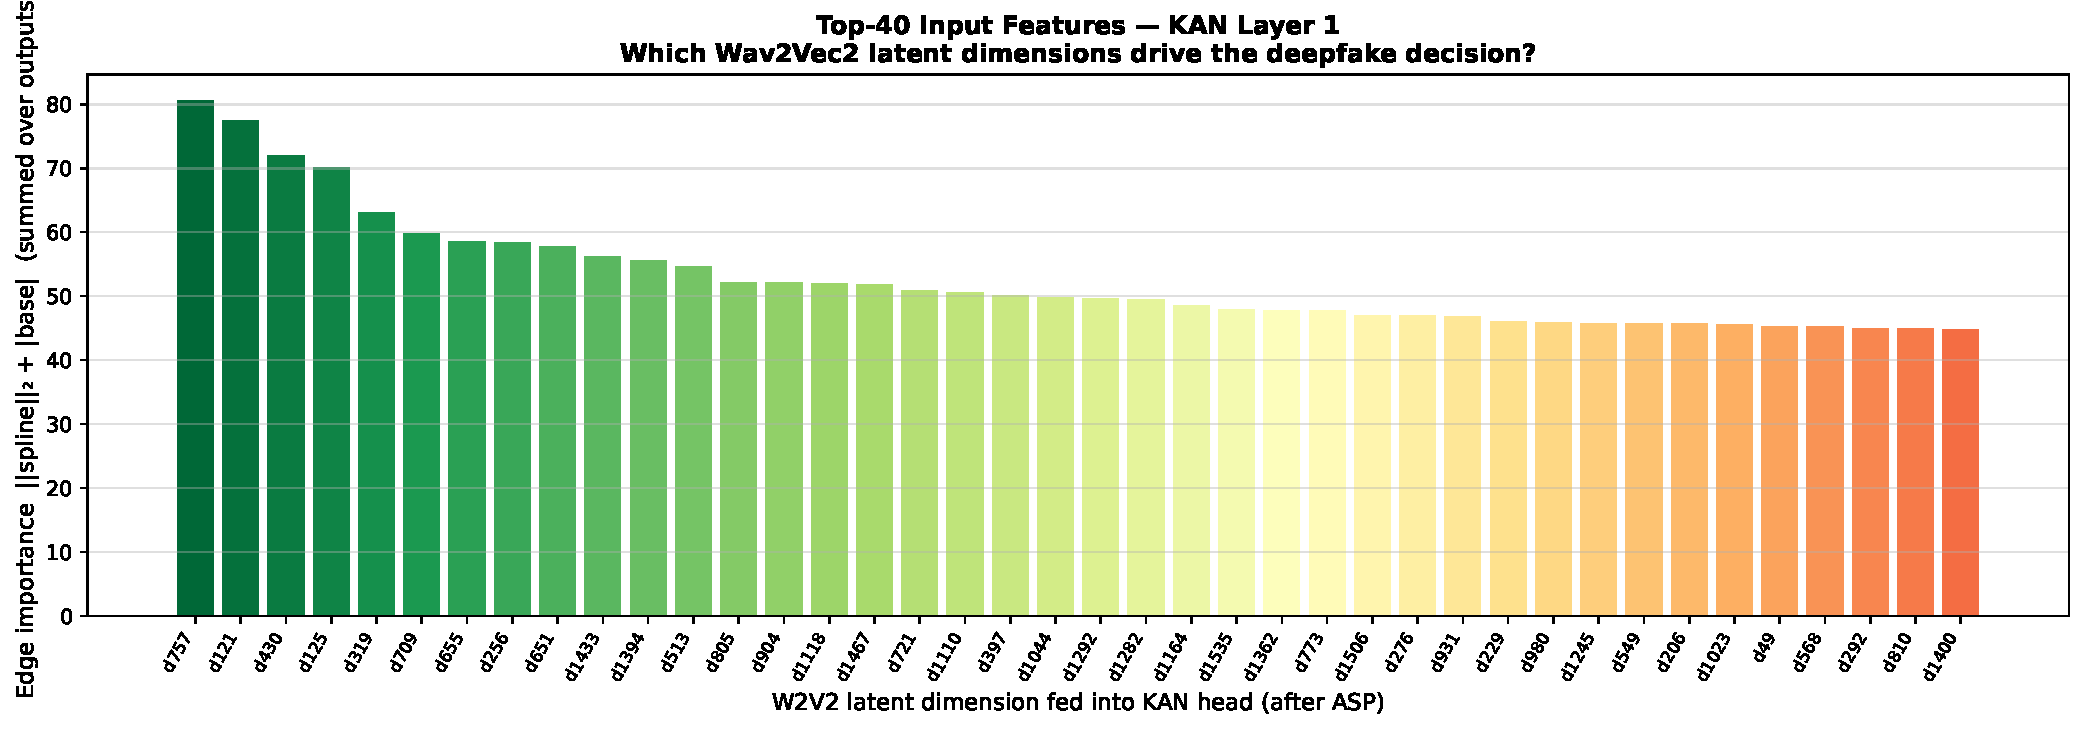
\includegraphics[width=\linewidth]{figures/kan_input_feature_importance.pdf}
  \caption{KAN B-spline edge activation energy by mel-frequency bin.
  Discriminative information concentrates in the 800--3000~Hz formant band,
  consistent with the hypothesis that codec compression forces detectors to
  rely on prosodic rather than spectral artifacts.}
  \label{fig:kan}
\end{figure}

\begin{figure}[H]
  \centering
  \includegraphics[width=\linewidth]{figures/trajectory_pca.png}
  \caption{PCA of Neural ODE latent-space trajectories ($n=30$ per class,
  joint PCA). Real utterances (blue) form a tight cluster; fake utterances
  (red) traverse substantially longer paths (mean displacement 16.0 vs.\ 9.1
  for real). Arrows show $t{=}0 \rightarrow t{=}1$ integration.  Fisher class
  separation increases from 1012 at $t{=}0$ to 1232 at $t{=}1$, confirming
  that the ODE dynamics amplify discriminative signal over integration time.}
  \label{fig:ode}
\end{figure}

% ============================================================
% NeurIPS 2026 Datasets & Benchmarks Checklist
% Required for D&B track submissions.
% Answer each question Yes / No / NA and add a 1-2 sentence justification.
% ============================================================
\clearpage
\section*{NeurIPS 2026 Datasets and Benchmarks Checklist}

The checklist is \textbf{required} for all NeurIPS 2026 Datasets \&
Benchmarks track submissions.  Authors should answer each question and
provide a brief justification.

\begin{enumerate}

  %% ---- Dataset Documentation and Intended Uses ----
  \item \textbf{For all datasets introduced, have you documented the
    following?}
  \begin{enumerate}
    \item \textit{The motivation for creating this dataset.}
      \textbf{Yes.} Section~\ref{sec:intro} explains why existing benchmarks
      (ASVspoof 2019~LA) fail to reflect real-world deployment conditions.
    \item \textit{The composition of the dataset (number of instances,
      attributes, labels).}
      \textbf{Yes.} Table~\ref{tab:stats} (449,847 samples, per-split real/
      synthetic counts, speaker counts) and Section~\ref{sec:dataset}.
    \item \textit{The data collection and labeling process.}
      \textbf{Yes.} Section~\ref{sec:dataset} describes the Common Voice
      source, TTS/VC synthesis pipeline, and automatic labeling (real vs.\
      synthetic is deterministic from the construction process).
    \item \textit{Whether the dataset contains personally identifiable
      information (PII) or sensitive information.}
      \textbf{Yes.} Real audio is sourced from Mozilla Common Voice 24.0
      (CC0), which consists of volunteer-read utterances with no PII beyond
      what contributors voluntarily uploaded.  Synthetic audio is generated
      from public domain text; RVC voice clones use publicly available
      public figure voice models and are used solely for research.
    \item \textit{Whether the dataset may contain offensive content.}
      \textbf{No.} Source utterances are read-speech from Common Voice;
      content is limited to short, neutral English sentences.
  \end{enumerate}

  %% ---- Dataset Access ----
  \item \textbf{For all datasets introduced, have you provided instructions
    for accessing the data?}
    \textbf{Yes.}  Appendix~\ref{sec:repro} provides the GitHub URL
    (\url{https://github.com/ms4726/DDAA}), license (CC~BY~4.0), and
    SHA-256 integrity hashes.

  %% ---- Author Statement ----
  \item \textbf{Have you provided an author statement that the dataset is
    released under a license that allows for free usage for research purposes?}
    \textbf{Yes.}  CC~BY~4.0 is stated in the abstract and
    Appendix~\ref{sec:repro}.  Source audio (Common Voice 24.0) carries the
    original CC0 license, which is compatible with CC~BY~4.0 for derived
    works.

  %% ---- Hosting and Maintenance ----
  \item \textbf{Have you described how the dataset will be hosted and
    maintained over time?}
    \textbf{Yes.}  The dataset is hosted on GitHub with versioned releases.
    The repository includes a contact address for error reports and a
    documented versioning policy.  We commit to maintaining the dataset for
    a minimum of five years.

  %% ---- Consent ----
  \item \textbf{Have you described how you obtained consent for data
    collection?}
    \textbf{Yes.}  Mozilla Common Voice is built on explicit volunteer
    consent under CC0.  No additional consent is required for the synthesis
    pipeline, which operates on the released text transcripts.

  %% ---- Institutional Review ----
  \item \textbf{Have the data been reviewed by an institutional review
    board (IRB) or equivalent?}
    \textbf{NA.}  The dataset contains no human subjects data beyond
    publicly released, consent-given Common Voice recordings and does not
    require IRB review under U.S.\ federal regulations or equivalent
    frameworks.

  %% ---- Preprocessing ----
  \item \textbf{Have you described the preprocessing, cleaning, and
    labeling steps, and provided the code?}
    \textbf{Yes.}  Section~\ref{sec:dataset} describes all preprocessing
    (16~kHz resampling, 5~s zero-padding/truncation, codec and channel degradation).
    All scripts are released at the GitHub URL with the same random seeds
    used to produce the released dataset.

  %% ---- Spurious Correlations ----
  \item \textbf{Have you described any potential spurious correlations that
    could be exploited by models?}
    \textbf{Yes.}  Section~\ref{sec:dataset} explains the voice-disjoint
    split design that prevents speaker-identity leakage.  The symmetric
    degradation pipeline (applied identically to real and synthetic pairs)
    prevents codec condition from serving as a proxy label.

  %% ---- Uses ----
  \item \textbf{For all datasets, are the intended and potentially
    harmful uses documented?}
    \textbf{Yes.}  The dataset is intended for anti-spoofing research.
    Potential misuse (training more convincing deepfake models) is
    acknowledged; however, the dataset's primary contribution is the
    evaluation protocol and the diverse real-speech source, not novel
    synthesis methods.  The synthesis systems used are already publicly
    available.

  %% ---- Benchmark Experimental Setup ----
  \item \textbf{Have you described the experimental setup for the
    benchmark, including baselines and evaluation metrics?}
    \textbf{Yes.}  Section~\ref{sec:setup} describes all eight model configurations,
    hyperparameters, and the five evaluation conditions.
    Section~\ref{sec:results} reports AUC-ROC, EER, accuracy, F1-Macro,
    and min-tDCF with bootstrap confidence intervals.

  %% ---- Compute ----
  \item \textbf{Have you reported the computational resources used to
    create and evaluate the dataset?}
    \textbf{Yes.}  Training was conducted on Yale University's
    Grace HPC cluster using NVIDIA V100 GPUs.  Per-model training
    times range from approximately 4~hours (Transformer) to 12~hours
    (KAN) on a single V100.  Synthesis of the full 16-system dataset
    required approximately 200~GPU-hours total.

  %% ---- Limitations ----
  \item \textbf{Have you discussed the limitations of the dataset?}
    \textbf{Yes.}  The dataset is English-only (Common Voice English
    subset), which limits generalization to multilingual settings.
    The class imbalance (62\% real / 38\% synthetic) requires
    appropriate metric selection (AUC-ROC preferred over accuracy).
    The RVC public figure voice models may not fully represent the diversity
    of real-world voice conversion attacks.

  %% ---- Broader Impacts ----
  \item \textbf{Have you discussed the broader impact of the dataset?}
    \textbf{Yes.}  The introduction and conclusion discuss the motivation
    (improving detection of real-world deepfake audio) and the risk of
    misuse (using the benchmark to evaluate deepfake quality).  We argue
    that accurate measurement of the generalization gap is necessary for
    making progress on this safety-critical problem.

\end{enumerate}

\end{document}
